\section{Contributions}
\begin{frame}{Contributions}

    The paper addresses the problem of \gbf{fairness} in \gbf{bipartite ranking models}, which have different requirements than classification models.
    
    The authors came up with \gbf{two contributions} to \gbf{improve fairness} of bipartite ranking models :
  \begin{itemize}
      \item AUC-based constraints
      \item ROC-based constraints
  \end{itemize}
  
  They show the \gbf{limitations} of the AUC-based constraints, and how the ROC-based constraints \gbf{address} them.
\end{frame}

\begin{frame}{Motivation}
    Fairness in ranking is important because it can have a significant impact on the decision-making process. For example, in the context of hiring, a biased ranking model can lead to unfair hiring practices.
\end{frame}


\subsection{AUC-based constraints}
\begin{frame}{AUC-based constraints}

\end{frame}

\begin{frame}{Limits of AUC-based constraints}
    \begin{figure}[t]
        \centering
        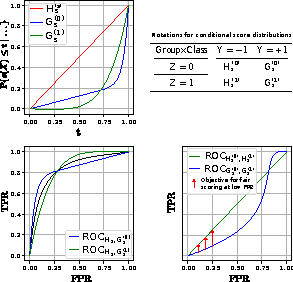
\includegraphics[width=0.6\columnwidth]{images/original_paper/example_simple_dists_explained_with_table2.pdf}
        \caption{Illustrating the limitations of $AUC$-based fairness.}
        \label{fig:example-1}
    \end{figure}
\end{frame}

\subsection{ROC based constraints}
\begin{frame}{ROC based constraints}
    small change
\end{frame}
